\section{Anpassung des Prozesses am Beispiel}
Eine kleine Gruppe Studenten wollte anhand einer Produkt-Idee das Prinzip des Sprints durchlaufen, da dieser Prozess sehr gefragt scheint. Bei dieser Idee handelt es sich um eine Online-Plattform für die Agrarbranche, wobei das Team noch ganz am Anfang der Konzeptfindung und Entwicklung steht. Diesbezüglich sollte der Sprint erste Ergebnisse liefern, ob die Idee beim Endkunden angenommen wird oder nicht. Allerdings stellte sich heraus, dass der Prozess, wie vorgegeben, für diesen Zweck nicht genau so umsetzbar ist. Der Ablauf der Sprints, sowie Abwandlungen sind im Folgenden genauer erläutert.
\subsection*{Tag 1}
\paragraph{Long Term Goal}
Der erste Tag startet mit einer sehr ertragreichen Gruppendiskussion zum Thema Projekt-Vision. Es wird schnell klar, dass bereits an dieser Stelle die Ansichten der einzelnen Team-Mitglieder teilweise stark voneinander abweichen. Nichtsdestotrotz ist es der Gruppe doch möglich, sich aufeinander abzustimmen und ein Long Term Goal aufzustellen, mit dem jeder Teilnehmer einverstanden ist.
%Gruppendiskussion
%Wo sehen wir uns in 6 Monaten? in 1 Jahr? in 5 Jahren?
%Warum wird das Projekt durchgeführt?
%
%Ziele:
%1/2 Jahr: Testbarer Prototyp
%1 Jahr: Beta-Version
%3 Jahre: Erweiterungen (Funktionalität, Branchen, Gebiete)
%Stichwortsammlung
%
%Resultat: Digitale und effiziente Plattform zur Ressourcenauslastung
\paragraph{Sprint-Fragen}
Weniger überraschend ist die Anzahl der Sprint-Fragen, die vom Team gestellt wurden. Besonders vor einer großen Aufgabe, wie dieser, treten viele Bedenken und Befürchtungen auf, welche im Rahmen dieser Aufgabe sehr schnell gesammelt werden können. Damit wird auch schnell klar, welche unterschiedlichen Teilbereiche das Gesamtprojekt zusätzlich anschneidet und in welchen Gebieten besondere Vorsicht geboten ist. Für das Team ist es in diesem Fall auch hilfreich zu verstehen, welche Risiken die einzelnen Teilnehmer sehen. An diesem Beispiel ist gut zu erkennen, dass es besonders zu Beginn eines solchen Projektes sehr viele offene Fragen gibt, von denen die Mehrzahl sicher nicht im Sprint behandelbar ist. Trotzdem fühlt es sich für das Team im Allgemeinen gut an, diese Bedenken an der Stelle festzuhalten und auch über den Workshop hinaus im Hinterkopf zu behalten. So entstehen beim Team AgriShare 16 Sprint-Fragen.

%Sammeln aller Fragen des Teams bezüglich des Projekts
%Risiken, Ängste...
%Annahmen und potentielle Hürden in Fragen umformulieren
%Die meisten Fragen sind vermutlich nicht im Sprint behandelbar, aber werden im Hinterkopf behalten.
%
%Resultat: 
%
%\begin{enumerate}
%	\item Wie ermöglicht man eine einfache Nutzung für ältere Personen?
%	\item Wie schaffe ich es, komplexe Vorgänge in einfache Schritte aufzubrechen?
%	\item Wie kriegen wir Kunden?
%	\item Wie kriegen wir loyale Beta-Tester?
%	\item Wie kann ich die Wetter-Daten sinnvoll einbauen?
%	\item Wie kann ich die Anwendung als komplette Service-Plattform auslegen?
%	\item Wie müssen wir das Design gestalten, um unsere Zielgruppe anzusprechen?
%	\item Wie können wir den rechtlichen Rahmen einhalten?
%	\item Wie verdienen wir Geld dabei?
%	\item Wie stellen wir sicher, dass alle benötigten Funktionalitäten abgedeckt sind?
%	\item Was macht uns besser als die Konkurrenz?
%	\item Wo sind die Hotspots?
%	\item Wie können wir unsere Corporate Identity auf die Zielgruppe abstimmen?
%	\item Wie bringen wir genug Startkapital auf? (mit/ohne Investoren)
%	\item Welche Kosten kommen auf uns zu?
%	\item Wie kann eine Vermittlung mit Verischerung durchgeführt werden?
%\end{enumerate}
\paragraph{Map}
Einfach
Kundenorientiert

Potential von Premium-Nutzern aufgekommen - wurde verworfen
Sehr lange Diskussionen und aneinander Vorbeireden
Unklarheit der Aufgabenstellung zu Beginn
Diskussion über Details, von denen jeder andere Ansichten hatte
Klassendiagramm konnte parallel dazu erstellt werden!
Eindeutige Begriffsbildungen!

Aufsbrechen des Gesamtprojekts in Einzelschritte
Gruppendiskussionen
Begriffsklärung sehr wichtig
\begin{figure}[h!]
	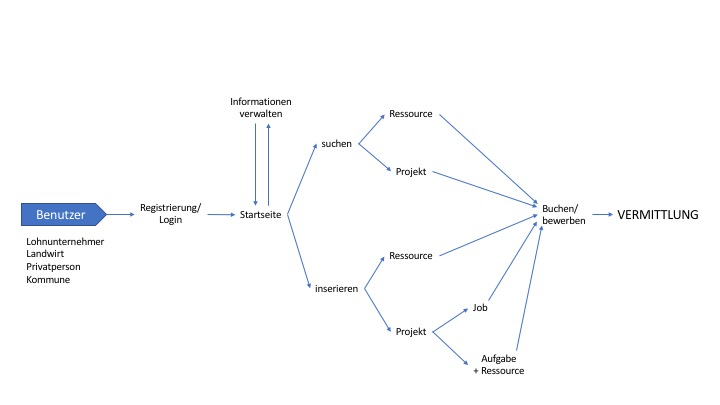
\includegraphics[width=\textwidth]{99_IMG/03_Sprint/map}
	\caption{Projekt Map}
	\label{fig:map}
\end{figure}

Wie in \ref{fig:map} dargestellt ist, wurden die Benutzer nochmal in Einzelgruppen eingeteilt. Das diente dem besseren Verständis im Team. Diese Benutzer müssen sich zuerst authentifizieren durch Login oder Registrierung. Danach sollen sie auf die Startseite geleitet werden, von wo aus sie verschiedene Möglichkeiten haben sollen. Die Nutzer können dann ihre Informationen verwalten, nach Inseraten suchen oder selber inserieren. Bei der Suche wird nur zwischen Ressourcen oder Projekten unterschieden, wohingegen ein Inserat ebenfalls eine Ressource oder ein Projekt beinhalten kann, dieses aber nochmal in Job oder Aufgabe unterteilt ist. Eine Aufgabe ist so definiert, dass es auch Ressourcen beinhalten kann. Nach diesen Abläufen kommt es typischerweise zu einer Buchung oder Bewerbung. Nach der Bestätigung wurde also eine Vermittlung durchgeführt, was das Ende des Prozesses beschreibt.

\paragraph{Ask the Experts}
Experten:
Theresa Jakob: Rechnungswesen
Matthias Coufal, Verena Schmöller: Ablauf der Buchung über Maschinenring
Sebastian Brunthaler: Typische Fehlerquellen in Projektteams
Landwirt: allgemeiner Eindruck des Projektes, Unklarheiten?
Masterand Horsch: Kundensicht

Rechnungswesen: 
Erhalten der Originalrechnung: Wenn per Post verschickt, Papierform ist Originalrechnung. Wenn per E-Mail verschickt, elektronische Form ist Originalrechnung (nicht der Ausdruck). 

Fehlerquellen:
Verschieben der Aufgaben von Person zu Person. Keine Verantwortung für eigene Aufgaben übernehmen.

Prozess MR:
Vermittlung der Maschinen/Dienstleistungen telefonisch. Meist nicht über MR, da sich Landwirte meist untereinander kennen. Abrechnung immer über MR, da der bürokratische Aufwand der Rechnungsstellung und Dieselbeihilfe abgenommen wird. Preis: Vorschläge von MR (Preiskatalog), aber individuell einstellbar.

Kundensicht: Möglichkeit, Maschinen mit Versicherung zu vermieten. Lohnunternehmer-Prozess bisher, allerdings mehr Potential in Privatpersonen, da sehr große Zielgruppe. Fokus auf kleineren Hausarbeiten

Da ein sehr hilfreicher potentieller Endkunde ebenfalls als Experte eingeladen wurde, welcher sehr viele Einsichten über potentielle Unklarheiten geben konnte, wurde der geplante Ablauf des Sprints bereits am Tag 1 abgewandelt. Es wurde der Fokus darauf gelegt, so viel wie möglich mit diesem Experten zu besprechen und die weiteren Punkte auf den nöchsten Tag zu legen.

Während aller Expertenrunden hat das restliche Team Notizen auf Klebezettel geschrieben und diese beiseite gelegt. Am Ende wurden alle Notizen gesammelt und an ein Whiteboard für alle sichtbar geklebt. Die geplanten weiteren Punkte wurden, wie bereits erwähnt, auf Tag 2 verschoben.

\paragraph{Logo und Name}
Parallel zum eigentlichen Sprint-Prozess war das Team an Tag 1 so motiviert, dass in den Pausen kleinere Diskussionen bezüglich Logo und Name des Produkts entstanden sind. Das hat dazu geführt, dass abends noch ein finales Logo und auch der letztendliche Produktname entstanden ist. 


\paragraph{Fazit}
Nach dem ersten Tag war das Gesamtfeedback des Teams sehr positiv. Der Prozess wurde bisher als sehr hilfreich angesehen, obwohl die Erwartungen im Vorfeld sehr niedrig waren. Unter Anderem war es möglich nur in einem Tag potentielle Risiken im Vorfeld zu eliminieren. Außerdem wurde vermutet, dass die Entwicklung allgemein erleichtert wurde, da viele Unklarheiten, welche sonst in der Implementierung Probleme gemacht hätten, bereits beseitigt wurden. Da das ganze Team fokussiert und konzentriert mitgearbeitet hat, war der gesamte Tag äußerst produktiv. So entstanden auch viele Ideen bezüglich möglicher Erweiterungen und weiterer Anwendungsgebiete. Auch vorher verworfene Anwendungsgebiete wurden wieder aufgerollt und ins Gedächtnis gerufen. Des Weiteren wurden sehr viele Bedenken des Teams schriftlich festgehalten, was das Team durchaus positiv stimmte. Im Allgemeinen entstanden sehr ertragreiche Diskussionen und Ideenfindungen. Es war auch sehr wichtig, die Erwartungen aller Teammitglieder aufeinander abzustimmen und sicherzugehen, dass alle die gleichen Ansichten haben. Dabei geht es nicht nur um zeitliche Erwartungen, sondern auch ganz allgemein was das Projekt überhaupt beinhaltet und was tatsächlich das Produkt darstellen soll. Denn jedes Teammitglied hatte für sich selbst ein sehr klares Bild von dem Projekt. Diese Ansichten waren allerdings sehr unterschiedlich von Person zu Person. Daher war Tag 1 vor allem auch im Bereich 'Teambuilding' sehr erfolgreich.

\subsection*{Tag 2}
Da am Tag 1 nicht alle geplanten Punkte abgearbeitet werden konnten, mussten die letzten drei Punkte am nächsten Tag behandelt werden.

\paragraph{Notizen sortieren}
Zuerst wurden die gesammelten Notizen sortiert. Dabei hat das gesamte Team zuerst Duplikate aussortiert und die restlichen Zettel in inhaltlich logische Gruppen eingeteilt. Für diese Gruppen wurden zusätzlich noch Überbegriffe festgelegt und ebenfalls an dem Whiteboard angebracht.

\paragraph{Notizen bewerten}
Anschließend wurden Sticker verteilt - zwei Sticker pro Person und 4 für den Decider. Jedes Teammitglied sollte sich nun das Long Term Goal, sowie die Sprint-Fragen erneut vor Augen führen. Danach werden die Sticker in einer stillen Abstimmung an die Notizen angebracht, die für den Sprint-Zeitraum als am Wichtigsten erachtet werden. Diese Notizen wurden dann an dem Whiteboard mit der Map angebracht, passend zu den jeweiligen Schritten.

\paragraph{Fokus des Sprints}
Nun war es die Aufgabe des Deciders, den Fokus für diesen Sprint einzugrenzen. Dabei sollten die Schritte auf der Map eingekreist werden, die in dieser Session abgearbeitet werden sollen. Da das PRojekt zu diesem Zeitpunkt noch am Anfang der Entwicklung stand, mussten für einen sinnvollen und testbaren Prototypen fast alle Bereiche der Map abgedeckt werden. Es handelt sich hierbei um ein komplett neues Produkt und nicht um ein einfaches Add-On oder eine Erweiterung. Deshalb wurde der Fokus auf die gesamte Map gerichtet, was in der Spezifikation nicht so vorgesehen ist. Jedoch hat der Decider entschieden, dass nur eine teilweise Prototypisierung des Projekts zu einseitige Ergebnisse hervorrufen würde und deshalb nicht sinnvoll ist.

\paragraph{Lighting Demos}
Liste mit für das Projekt interessante Produkte

Liste:
\begin{itemize}
	\item Airbnb
	\item Google Maps
	\item Uber
	\item Tractorpool
	\item ...
\end{itemize}

Jedes Teammitglied hat sich mit 2-3 Produkten beschäftigt und für das Projekt relevante Teile herausgefunden. Dabei wurde nicht nur auf besonders gute Umsetzungen geachtet, sondern auch als nicht so gut erachtete Bausteine hervorgehoben. 
Die Übung wurde allgemein als eine sehr gute Inspiration erachtet und es gab nur wenige Diskussionen. 
Die Ergebnisse jeder Person hat diese in einer kurzen Demo vor dem ganzen Team vorgetragen und ist dabei auf alle wichtigen Details eingegangen. 
Dabei ist aufgefallen, dass zwar das meiste schon im Vorhinein bekannt war, allerdings nicht jeder diese Dinge als besonders gut gesehen hat.

App reiner Assistent (nicht volle Funktionalität)


\paragraph{Aufgabenverteilung}
Die Aufgaben verteilung erfolgte ziemlich reibungslos, da sich das Team sehr schnell darauf geeinigt hatte, wer welche Bereiche bearbeiten soll. Da der Fokus in diesem Fall sehr breit gefächert war, wurden jeder Person jeweils 3 Schritte zugeteilt.

\paragraph{Sketch}
Bereits nach den ersten 30 Minuten der Ideensammlung ist aufgefallen, dass der Prozess so nicht hilfreich für das Projekt ist. Es wurden zu viele Screens für den Prototypen benötigt, wie in der kurzen Zeit von wenigen Personen erstellt werden konnten. Außerdem war es besonders wichtig, dass die Screens eine einheitliche Maske und einen einheitlichen Aufbau hatten. Deshalb war es weniger sinnvoll, jede Person ein eigenes Set an Bildschirmen bauen zu lassen. Nachdem also jeder eigenen Ideen gesammelt hat, wurde begonnen, die Screens groß auf einem Whiteboard zu erstellen in einer Gruppendiskussion. Da fiel auf, dass es immer noch sehr viele Unklarheiten bezüglich der grundlegenden Funktionsweise gab. Das Team führte sich allerdings immer wieder vor Augen, dass das Endprodukt nicht besonders ausgeflippt oder kreativ gestaltet sein muss, sondern einfach zu verstehen und nach einem einheitlichen Prinzip aufgebaut sein soll. Innerhalb des Nachmittags von Tag 2 hat es das Team geschafft, eine einheitliche Maske zu erstellen und es konnte die Startseite, sowie teilweise die Kartenansicht erstellt werden.
Zugunsten des Gesamtteams und des Projekterfolges wurde am Ende von Tag 2 beschlossen, die Screens nach einem eigenen Prozess in Gruppendiskussion zu erstellen, anstatt dem Sprint-Prozess zu folgen.

\paragraph{Fazit}
Am Ende von Tag 2 war das Team wiederum einer Meinung, was den Gesamtprozess angeht. Der Sketch-Prozess, wie spezifiziert, ist nicht sinnvoll für ein einheitliches Produkt mit vielen Screens. Das heißt nicht, dass die Herangehensweise grundsätzlich als falsch angesehen wurde. Für kleinere Add-Ons, Zusatzfunktionen oder Design-Fragen könnte dies durchaus einen großen Mehrwert gegenüber "unserer" Herangehensweise haben. Nichtsdestotrotz war das Projektteam trotzdem sehr kreativ und fokussiert bei der Sache. Auch die Meinung von Nicht-Teammitgliedern war durchaus wertvoll, was durch verschiedene Besucher zum Ausdruck kam. Da die Befürchtung aufkam, man könnte sich an unnötigen Details aufhängen, konnte im Nachhinein gesagt werden, dass dies immer sehr gut eliminiert werden konnte. Da zu diesem Zeitpunkt bereits der komplette Sprint-Prozess abgewandelt worden ist, sind die Rollen natürlich auch ineinander verschmolzen.

\subsection*{Tag 3}
Der Tag wurde so begonnen, wie der Tag zuvor beendet wurde. Nach und nach Aufbauen der verschiedenen Screens des Endproduktes. Um Zeit einzusparen, hat ein Teammitglied parallel dazu schon die Prototypen der erstellten Bildschirme erstellt.

\subsection*{Tag 4}
Bereits zu Beginn von Tag 4 war klar, dass es wenig Sinn macht, die Screens so zu testen, da sie einfach noch zu wenig Aussagekraft haben. Deshalb wurde beschlossen, dass die geplanten Tests verschoben werden und direkt nach dem Sprint damit begonnen wird, das Produkt zu implementieren. Ein weiterer Grund dafür, die Tests abzusagen, war, dass ein Usertest mit unserer Zielgruppe zu viel Aufwand für einen Tag wäre. Denn Landwirte sind vor allem im Sommer immer sehr beschäftigt und können nicht für 30 Minuten in die Stadt fahren. Deshalb wurde beschlossen, zu einem späteren Zeitpunkt potentielle Tester zu besuchen und dort zu testen.

\subsection*{Tag 5}
Am letzten Tag waren immer noch nicht alle Screens gezeichnet, aber die Energie des Teams war mittlerweile sehr niedrig. Deshalb wurde die restliche Zeit genutzt, um nochmal alle Details zu klären, die restlichen Screens zu erstellen und sich auf ein Logo und einen Namen zu einigen. Dieses Ziel wurde erreicht und das Team hat den Sprint mit einem sehr guten Gefühl abgeschlossen.

\subsection*{Allgemeines Fazit - Sprint}
Wie bereits oben angedeutet, hatte das Projektteam allgemein sehr niedrige Erwartungen an den Prozess. Es wurde kein großer Mehrwert erwartet, weshalb am Ende jeder sehr positiv überrascht von dem Ergebnis war. Hauptsächlich die ersten beiden Tage haben dem Team vermutlich sehr viel Arbeit und zukünftige Diskussionen erspart. Sehr positiv anzumerken ist, dass jeder Beteiligte sehr konzentriert mitgearbeitet hat und mit großem Arbeitswillen bei der Sache war. Das führte dazu, dass das Team während der ganzen 5 Tage in einem Flow war dementsprechend sehr gute Arbeit geleistet und konstruktive Beiträge geleistet hat. Allerdings ist auch aufgefallen, dass der Prozess, wie vorgesehen, nicht sinnvoll für ein komplett neues Produkt ist. Dies beinhaltet zu viele Einzelteile und zu viele Details, die das ganze Team zusammen abklären muss. Durchaus sinnvoll wäre das für eine Erweiterung eines bestehenden Produktes. In der abgewandelten Variante dieses Teams wurden auch viel mehr Ergebnisse erzielt als erwartet. In nur fünf Tagen konnte ein Konzept erstellt werden, alle Screens des Produktes gezeichnet werden und sich auf ein Logo und einen Brand-Name geeinigt werden. Da alle Teammitglieder hauptberuflich andere Dinge machen, wie ein Studium oder Vollzeitarbeit, hätte es ohne den Sprint wohl sehr lange gedauert, bis diese Dinge geklärt worden wären. \\
Diesbezüglich war sich das Team auch einig, einen Follow-Up Sprint zu starten, sobald das Grundprodukt implementiert ist und erste User-Tests gemacht wurden. 